\documentclass[12pt]{article}
\usepackage[utf8]{inputenc}
\usepackage[left=2cm,right=2cm,top=2cm,bottom=2cm]{geometry}
\usepackage{graphicx, amsmath, listings, xcolor}
\usepackage[small]{caption}
\usepackage{subcaption}
\usepackage[spanish]{babel}
\usepackage{url}
\setlength{\parskip}{\baselineskip}
\graphicspath{ {images/} }
\spanishdecimal{.}

\usepackage{hyperref}
\hypersetup{
	colorlinks=true,
	linkcolor=blue,     
	urlcolor=blue,
	citecolor=blue,
}


\begin{document}

	\thispagestyle{empty}

	\begin{center}
		{\Large \bf Pruebas estadísticas}\\
		Gabriela S\'anchez Y.\\
		5064
	\end{center}
 
	Esta práctica se divide en dos partes, una teórica y una práctica. La parte teórica consiste en contestar una serie de preguntas relacionadas con pruebas estadísticas, mientras que la práctica muestra la aplicación de las mismas al un conjunto de datos de {\em seguridad pública y justicia} obtenidos del INEGI \cite{inegi}. 


	\section{Parte teórica}
	
	En esta sección se responde una serie de preguntas realizando una lectura previa sobre pruebas estadísticas en tres sitios: \href{https://help.xlstat.com/s/article/que-es-una-prueba-estadistica?language=es#:~:text=Una\%20prueba\%20estad\%C3\%ADstica\%20es\%20una,nula\%2C\%20y\%20suele\%20denominarse\%20H0.&text=H0\%20normalmente\%20se\%20opone\%20a,alternativa\%2C\%20denominada\%20H1\%20o\%20Ha}{Centro de Ayuda XLSTAT}, \href{https://www.ecured.cu/Pruebas_estad\%C3\%ADsticas}{EcuRed} y \href{https://www.maximaformacion.es/blog-dat/guia-para-encontrar-tu-prueba-estadistica/}{Máxima formación}.
	
	\noindent {\bf Relación entre contraste de hipótesis y pruebas estadísticas}
	
	Ambas formulan hipótesis y evalúan la evidencia estadística que proporcionan los datos para aceptar o rechazar dichas hipótesis. 
	
	\noindent {\bf ¿Qué indicaría rechazar la hipótesis nula?}
	
	Para poder rechazar una hipótesis nula, es necesario que el $p$-valor obtenido de la prueba estadística aplicada sea menor que el nivel de significación $\alpha$ de la misma. Al rechazar la hipótesis nula, se acepta la hipótesis alternativa.
	
	
	\noindent {\bf ¿Cómo se interpreta la salida de una prueba estadística?}
	
	Antes de realizar la prueba se debe especificar un nivel de significación $\alpha$, este valor indica la probabilidad de rechazar la hipótesis nula cuando es verdadera (error de tipo I). Para interpretar la salida de la prueba, se compara el $p$-valor con el valor de $\alpha$: si $p$-valor $< \alpha$, se rechaza la hipótesis nula $H_0$; en cambio, si $p$-valor $> \alpha$ no se rechaza la hipótesis nula. Este último resultado no necesariamente implica que se debe aceptar la hipótesis nula, más bien se tiene que no existe suficiente evidencia estadística para rechazar dicha hipótesis.
	
 	\noindent {\bf ¿Cómo seleccionar el valor de $\alpha$?}
 	
 	Anteriormente se mencionó que $\alpha \in [0, 1]$ indica la probabilidad de rechazar la hipótesis nula cuando ésta es verdadera, por lo que la elección de su valor depende de los datos que se estudian. El qué tan peligroso es cometer un error de este tipo, determinará el valor de $\alpha$ a usar. Por ejemplo, si se desea analizar el efecto de algún tratamiento médico, el valor elegido debe ser muy pequeño. 
 	
	\noindent {\bf ¿Cuáles son los errores frecuentes de interpretación del $p$-valor?}
	
	Tomar un valor de significación no adecuado, conduciría a cometer el error de rechazar la hipótesis nula cuando ésta es verdadera.
	 
	\noindent {\bf ¿Qué es la potencia estadística y para qué sirve?}
	
	La potencia de una prueba estadística es la capacidad de la prueba para rechazar la hipótesis nula cuando la hipótesis alternativa es verdadera. En otras palabras, la potencia es la probabilidad de no cometer un error de tipo II. Es por esto que su valor es $1-\beta$, donde $\beta$ es la probabilidad de aceptar la hipótesis nula cuando es falsa (error de tipo II).
	
	Tener un buen valor para la potencia estadística, indica que la prueba detectará un efecto que realmente existe en los datos. 
	
	\noindent {\bf ¿Cuáles son los supuestos para aplicar técnicas paramétricas?}
	
	Se usa una prueba paramétrica si los datos son cuantitativos. Un requisito indispensable es que los datos tengan una distribución de probabilidad normal, además deben tener varianzas iguales o similares (homocedasticidad).
	
	\noindent {\bf Ejemplos de pruebas estadísticas paramétricas y no paramétricas}
	
	Dentro de las pruebas paramétricas más comunes se encuentran la prueba $t$ de Student que se utiliza para comparar las medias de dos poblaciones, el análisis de varianza (ANOVA), el análisis de covarianza (ANCOVA), entre otros.
	
	Algunos ejemplos de pruebas no paramétricas son la prueba de Wilcoxon que se puede usar para comparar las medias de dos grupos que no siguen una distribución normal, Kruskal-Wallis (el equivalente a un ANOVA de una vía) y para comparar dos grupos de variables cualitativas nominales y ordinales se puede usar la prueba Chi-cuadrada.  
	
	\noindent {\bf Guía para encontrar la prueba estadística que buscas}
	
	 

	\section{Parte práctica}
	
	En esta sección se aplican distintas pruebas estadísticas usando el lenguaje de programación \textsc{R} \cite{rstatistics} a los datos sobre {\em seguridad pública y justicia} obtenidos de la página del Instituto Nacional de Estadística y Geografía \cite{inegi}. Para todas las pruebas se fija el nivel de significación $\alpha = 0.05$.
	
	\subsection{Prueba de Shapiro}
	
	La prueba de {\em Shapiro} es usada para determinar si una muestra sigue una distribución normal. La hipótesis nula $H_0$ de esta prueba es que los datos de la muestra están normalmente distribuidos. Si el $p$-valor es mayor que $\alpha$, no se rechaza la hipótesis nula y en este caso se confirma que la muestra cumple con la normalidad. En las siguientes subsecciones se muestran algunos ejemplos prácticos del uso de esta prueba.
	
	\subsection{Prueba t de una muestra}
	
	Es una prueba paramétrica usada para determinar si la media de una muestra (con distribución normal), podría tener un valor específico.
	
	Se toman los datos de la tasa de prevalencia delictiva por cada cien mil habitantes en las distintas entidades federativas del país en los años 2010 a 2013 y se verifica con la prueba si se cumple la hipótesis $H_0$ que la población tiene una media igual a 23,600. Antes de aplicar la prueba se verifica que los datos sigan una distribución normal con la prueba de {\em Shapiro}. A continuación se muestran los resultados obtenidos de ambas pruebas.
	\begin{verbatim}
		Shapiro-Wilk normality test
	
	data:  delitos
	W = 0.97897, p-value = 0.1259
	--------------------------------------
		One Sample t-test
	
	data:  delitos
	t = 0.022397, df = 95, p-value = 0.9822
	alternative hypothesis: true mean is not equal to 23600
	95 percent confidence interval:
	22456.15 24769.96
	sample estimates:
	mean of x 
	23613.05 
	\end{verbatim}

	El $p$-valor obtenido de la prueba de {\em Shapiro} indica normalidad. Por otra parte, el $p$-valor obtenido de la prueba $t$ indica que no se puede rechazar la hipótesis nula, sin embargo esto no quiere decir que se acepte. Es decir, esto no afirma que la media de los datos sea 23,600. 
	
	\subsection{Prueba de los rangos con signo de Wilcoxon}
	
	Es la alternativa a la prueba anterior cuando no se cumple con la distribución normal.
	
	Se analiza si la media de los datos de la tasa de prevalencia delictiva en el periodo comprendido desde 2010 hasta 2019 en todas las entidades federativas del país es igual a 23,600. Antes de aplicar la prueba, se verifica si hay normalidad en los datos. La salida que se obtiene es la siguiente:
	\begin{verbatim}
		Shapiro-Wilk normality test
	
	data:  todos_delitos
	W = 0.94654, p-value = 9.857e-09
	-----------------------------------------
		
		Wilcoxon signed rank test with continuity correction
	
	data:  todos_delitos
	V = 23976, p-value = 0.02514
	alternative hypothesis: true location is not equal to 23600
	\end{verbatim}

	El $p$-valor obtenido es menor a $\alpha$, por lo que se rechaza la hipótesis nula y se acepta la hipótesis alternativa que la media de los datos no es igual a 23,600.
	
	\subsection{Prueba t para dos muestras y prueba de suma de rangos de Wilcoxon} \label{wilcox-2}
	
	Las dos pruebas son usadas para comparar las medias de dos muestras. La diferencia radica en que la prueba $t$ requiere que se cumpla la normalidad, mientras que la prueba de {\em Wilcoxon} no.
	
	Ahora se analiza si la media de la tasa de prevalencia delictiva en el periodo comprendido desde 2010 hasta 2019 en la zona norte del país es igual a la de la zona centro. Para la zona norte se consideran únicamente los estados que están en la frontera del país; es decir, Baja California Norte, Coahuila, Chihuahua, Nuevo León, Sonora y Tamaulipas. Para la zona centro se consideran también seis entidades federativas: Ciudad de México, Guanajuato, Estado de México, Michoacán, Querétaro y Tlaxcala.
	
	Como primer paso se revisa si ambas muestras cumplen con la normalidad y de acuerdo a los $p$-valores obtenidos, se concluye que una de ellas no lo cumple. Es por esto que se utiliza la prueba de suma de rangos de {\em Wilcoxon}. 
	\begin{verbatim}
		Shapiro-Wilk normality test
	
	data:  norte
	W = 0.96785, p-value = 0.1548
	-------------------------------
		Shapiro-Wilk normality test
	
	data:  centro
	W = 0.92417, p-value = 0.002158
	\end{verbatim}
	
	El $p$-valor obtenido de la prueba de suma de rangos de {\em Wilcoxon} es mayor que el valor de $\alpha$ por lo que se concluye que no existe suficiente evidencia estadística para rechazar dicha hipótesis nula.
	\begin{verbatim}
	Wilcoxon rank sum test with continuity correction

	data:  norte and centro
	W = 1298, p-value = 0.3271
	alternative hypothesis: true location shift is not equal to 0
	\end{verbatim} 
	
	Sin embargo, si se grafica un diagrama de caja-bigote de ambas muestras tal y como se observa en la figura \ref{boxplot-zonas}, es claro que las muestras no tienen la misma media.
	
	\begin{figure}
		\centering
		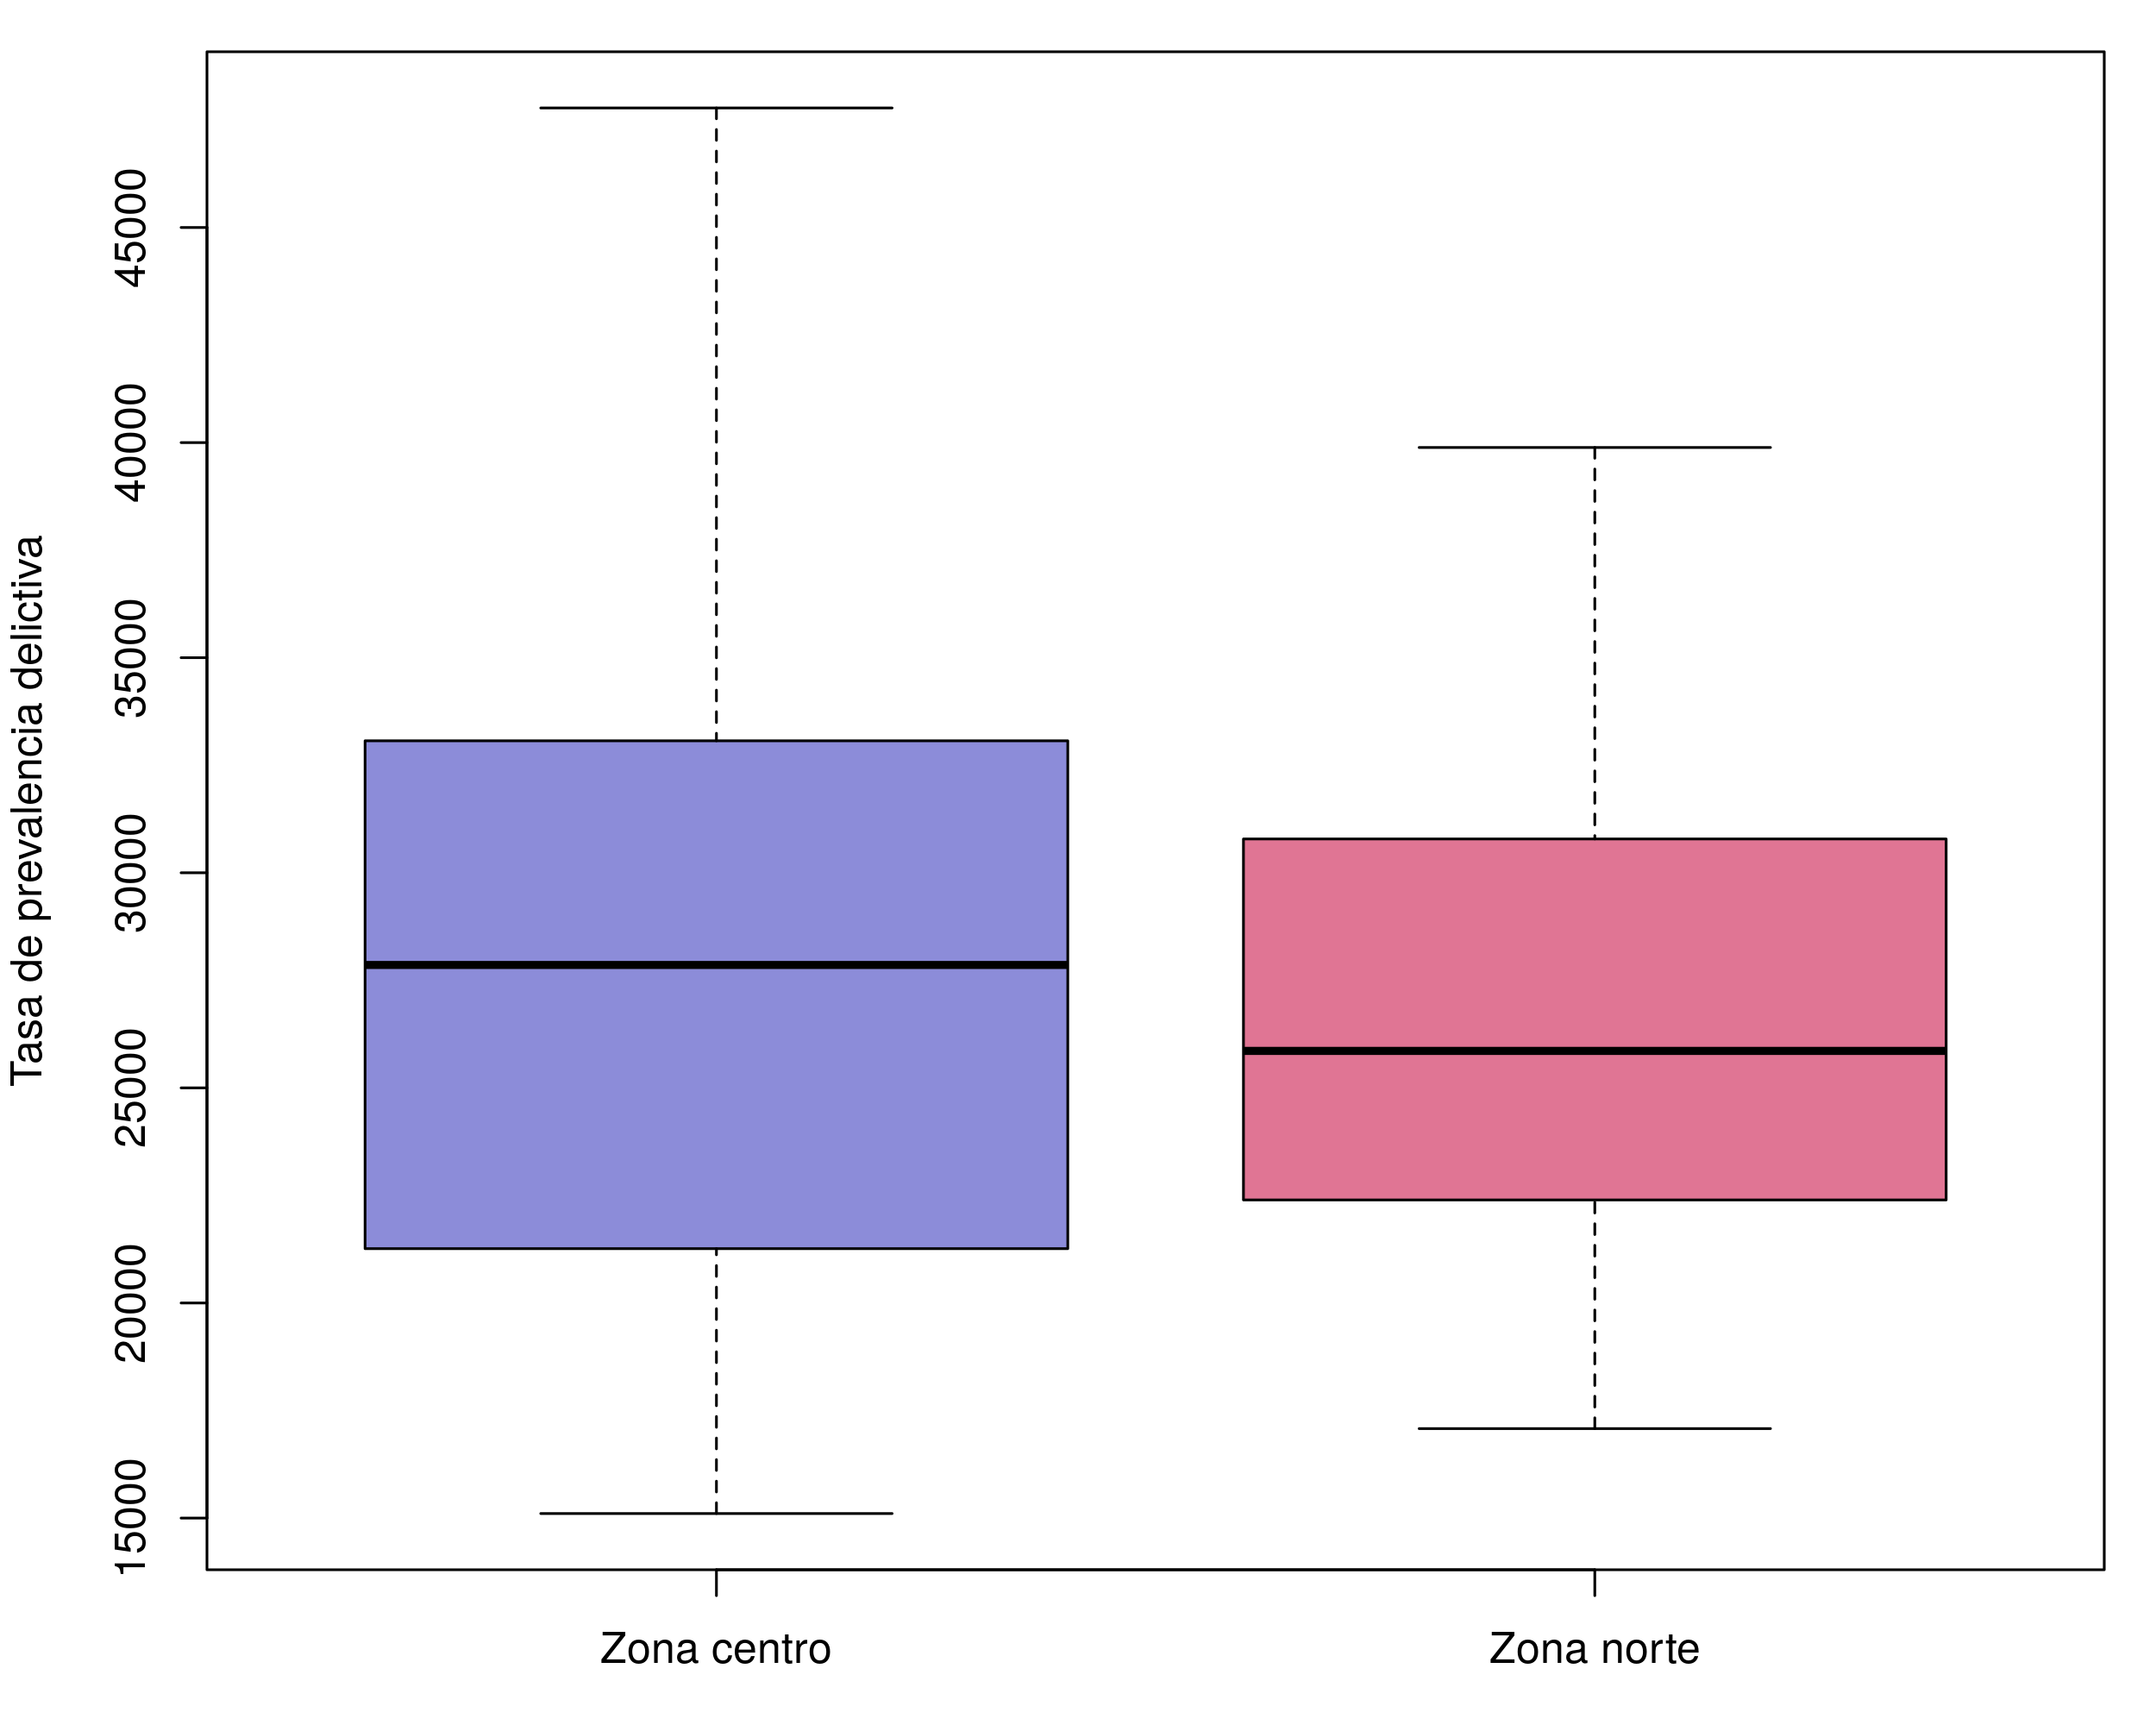
\includegraphics[scale=0.5]{boxplot_norte-centro.png}
		\caption{Diagrama caja-bigote de la variación de la tasa de prevalencia delictiva en distintas zonas del país.}
		\label{boxplot-zonas}
	\end{figure}

	\subsection{Prueba de Kolmogorov-Smirnov}
	
	Esta prueba es utilizada para determinar si dos muestras siguen la misma distribución. La hipótesis nula $H_0$ de esta prueba es precisamente que ambas muestras provienen de la misma distribución.
	
	\subsection{Prueba de Fisher}
	
	Es usado para determinar si dos muestras tiene la misma varianza. Para un ejemplo de su uso, se retoman las muestras utilizadas en la subsección \ref{wilcox-2}. El resultado obtenido de aplicar la prueba es el siguiente:
	\begin{verbatim}
		F test to compare two variances
	
	data:  centro and norte
	F = 2.1669, num df = 53, denom df = 53, p-value = 0.00564
	alternative hypothesis: true ratio of variances is not equal to 1
	95 percent confidence interval:
	1.257380 3.734393
	sample estimates:
	ratio of variances 
	2.166922 
	\end{verbatim}

	Vea que se cumple que $p$-valor $< \alpha$, por lo que se rechaza la hipótesis nula y se acepta la hipótesis alterna que las varianzas son distintas.
	
	\subsection{Prueba Chi cuadrada}
	
	Esta prueba se usa para determinar si dos características son independientes o tienen alguna asociación. 
	
	Para ejemplificar esta prueba se toman los resultados de percepción de la población mayor de 18 años, por tipo de autoridad. Se tienen dos tipos de percepción {\em algo efectivo} y {\em muy efectivo} y se analizan sólo tres tipos de autoridad: policía federal, estatal y municipal. Los datos se muestran en el cuadro \ref{dtaos-chi}.
	
	\begin{table}[b]
		\centering
		\caption{Percepción de la efectividad del trabajo de diferentes tipos de autoridades.}
		\label{dtaos-chi}
		\begin{tabular}{lrr}
			\hline
			 & Muy efectivo & Algo efectivo\\
			\hline
			Policía federal & 16.3 & 49.7 \\
			Policía estatal & 8.7 & 45.1 \\
			\hline
		\end{tabular}
	\end{table}
	
	Con estos datos, se desea saber si el tipo de autoridad afecta al nivel de percepción. La hipótesis nula es que no hay asociación entre estas dos variables, es decir, que el tipo de autoridad no se asocia con la percepción de efectividad. Los resultados obtenidos se muestran a continuación.
	\begin{verbatim}
		Pearson's Chi-squared test

	data:  prueba
	X-squared = 1.3047, df = 1, p-value = 0.2534
	\end{verbatim}
	
	El $p$-valor es mayor que el nivel de significación, lo que significa que no se puede rechazar la hipótesis nula. Para analizar el valor de {\em chi cuadrada}, primero se aclara que se tiene una tabla de valores de $2 \times 2$, es decir, se tienen dos grados de libertad. En este caso el valor crítico con el que se compara el valor de {\em chi cuadrada} es 3.841. Observe que {\em chi cuadrada} < 3.841, de acuerdo a esto, la hipótesis nula no se rechaza.
	
\bibliographystyle{plain}
\bibliography{biblio}

\end{document}

